\documentclass[11pt,a4paper]{article}
\usepackage{a4wide,url,graphicx,wrapfig}
\usepackage[utf8]{inputenc}
\usepackage[russian]{babel}

\parindent0pt
\parskip3pt

\title{Человек и Техническая Система. } 

\author{Николай Шпаковский}

\date{20 января 2003}

\begin{document}
\maketitle

\begin{quote}
  Часть I. \url{http://www.gnrtr.ru/Generator.html?pi=201&cp=3}
\end{quote}

\section*{Человек – это часть Технической Системы или нет?}

\begin{flushright}
  \ldots{} последние слова книги пророка Люстрога гласят: «все истинно верующие
  да разбивают яйца с того конца, с какого удобнее». \\ 
  Джонатан Свифт «Путешествия Гулливера» 
\end{flushright}

\section*{Введение}
Теория Решения Изобретательских Задач (ТРИЗ), разработанная талантливым
инженером, изобретателем и гениальным выдумщиком Г.С. Альтшуллером, широко
известна и, несомненно, является наиболее эффективным инструментом решения
инженерных задач в настоящее время. Опубликовано большое количество материалов
на русском и английском языках, в которых суть теории раскрывается достаточно
полно для первоначального знакомства с ней. Лучшим русскоязычным ресурсом
является сайт Минского центра
ОТСМ-ТРИЗ\footnote{\url{http://www.trizminsk.org}}, лучшим англоязычным –
Американский ТРИЗ-Журнал\footnote{\url{http://www.triz-journal.com}}.  Изучив
ТРИЗ по книгам и статьям, можно легко учить других – материал настолько
богатый и увлекательный, что интерес к занятиям будет обеспечен.

Однако, для более глубокого понимания ТРИЗ необходимо тщательное осмысление
изложенного материала, в первую очередь, понятий и терминов ТРИЗ. Ведь многое
в ТРИЗ изложено, как материал для дальнейших размышлений, а не набор
информации для простого запоминания.

За время работы для компании САМСУНГ в качестве ТРИЗ-консультанта мне пришлось
заново и всерьез переосмыслить все то, что я знал о ТРИЗ раньше. При решении
технических задач, обходе патентов конкурирующих компаний и разработке
прогноза развития технических систем очень важно было понять глубинное
содержание каждого термина ТРИЗ с тем, чтобы применять ее инструменты с
максимальной эффективностью.

Одним из основных понятий в ТРИЗ и одним из важнейших звеньев всех без
исключения ее инструментов является понятие «Техническая Система». Этот термин
вводится в классической ТРИЗ без определения, как производное от понятия
«Система». Но при ближайшем рассмотрении становится ясно, что это понятие –
«Техническая Система» – требует дальнейшей конкретизации. В пользу такого
утверждения говорит, например, семантический аспект. Понятие «Техническая
Система» переводится с русского языка на английский двумя способами:
«Technical System» и «Engineering System». Используя любую поисковую систему в
Интернете, легко убедиться, что эти понятия в понимании специалистов,
проявляющих активность в ТРИЗ, практически равноценны. Или взять, к примеру,
глоссарий Виктора
Фея\footnote{\url{http://www.triz-journal.com/archives/2001/03/a/index.htm}},
в котором просто нет разъяснения ни того, ни другого понятия.

В настоящей статье я попытался описать мое осмысление термина «Техническая
Система», постепенно сложившееся после того, как для решения конкретной задачи
мне понадобилось узнать полный состав минимально работоспособной технической
системы.

\section*{Попытка анализа понятия «Техническая Система»}

Для начала рассмотрим, что же такое система вообще.  Имеется много разных
определений системы. Самое залихватское, абстрактное, потому абсолютно
исчерпывающее, но малопригодное для практических целей определение дал
В. Гейнс [1]: \textbf{«Система – это то, что мы определим как систему»}. На
практике чаще всего пользуются определением системы А. Богданова [2]:
\textbf{«Система – это множество взаимосвязанных элементов, обладающих общим
  (системным) свойством, не сводящимся к свойствам этих элементов»}.

А что такое «Техническая Система»? 

К сожалению, непосредственно понятие «Техническая Система» у Г. Альтшуллера не
определено. Из контекста ясно, что это некоторая система, имеющая отношение к
технике, техническим объектам. Косвенным определением Технической Системы (ТС)
могут служить сформулированные им три закона, вернее, три условия, которые
должны удовлетворяться для ее существования [3]:

\begin{itemize}
\item[1.] Закон полноты частей системы. 
\item[2.] Закон «энергетической проводимости» системы. 
\item[3.] Закон согласования ритмики частей системы. 
\end{itemize}
Согласно закону полноты частей системы каждая ТС включает в себя, как минимум,
четыре части: двигатель, трансмиссию, рабочий орган и систему управления.
\begin{center}\small
  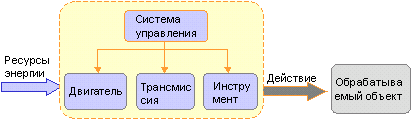
\includegraphics[width=.6\textwidth]{mts-1.png}\\
  Минимальная структура работоспособной Технической Системы по Г. Альтшуллеру.
\end{center}
То есть, имеется какая-то система, машина, состоящая из технических объектов,
подсистем, которая может выполнять требуемую функцию. Она включает рабочий
орган, трансмиссию и двигатель. Все, управляющее действием этой машины,
помещается в «Систему управления» или малопонятную «Кибернетическую часть»
[4].

Важным здесь является понимание того, что ТС создается для выполнения
некоторой функции. Наверное, следует понимать так, что минимально
работоспособная ТС может выполнять эту функцию в любой момент, без
дополнительного доукомплектования. Подходы к определению Технической Системы
представлены в книге «Поиск новых идей» [5], где приводится определение
«Развивающейся Технической Системы». Этого вопроса касается в своих интересных
исследованиях В. Королев [6,7]. Некоторые критические замечания посвящены
этому и в материалах Н. Матвиенко [8]. Определение же понятия «Техническая
Система» применительно к ТРИЗ приведено в книге Ю.Саламатова [9]:
\begin{quote}\bf
  «Техническая Система – это совокупность упорядоченно взаимодействующих
  элементов, обладающая свойствами, не сводящимися к свойствам отдельных
  элементов и предназначенная для выполнения определенных полезных функций».
\end{quote}

Действительно, у человека есть какая-то потребность, для удовлетворения
которой надо выполнить некоторую функцию. Значит, нужно каким-то образом
организовать систему, эту функцию выполняющую, – Техническую Систему – и
удовлетворить потребность.

Что же смущает в приведенном выше определении Технической Системы? Не совсем
понятное слово «предназначенная». Наверное, все-таки здесь важнее не чьи-то
пожелания, а объективная возможность выполнения требуемой функции.
\begin{quote}\it
  Например, для чего предназначен металлический цилиндр с осевым отверстием
  переменного диаметра и резьбой на одном его конце?

Ответить на такой вопрос практически невозможно. Дискуссия сразу переходит в
плоскость вопроса «а где это можно было бы применить?».
\end{quote}

Но можно ли, пользуясь этим определением, сказать: пока это еще не Техническая
Система, а с этого момента – уже Техническая Система? Написано так: «....ТС
появляется, как только технический объект приобретает способность выполнять
Главную Полезную Функцию без человека». А дальше сказано, что одна из
тенденций развития ТС – это удаление человека из ее состава. Значит, на
каком-то этапе развития ТС человек является ее частью. Или нет?
Непонятно.....
\begin{quote}\it
  Наверное, мы ни в чем не разберемся, если не найдем ответа на следующий
  вопрос: человек – это часть Технической Системы или нет?
\end{quote}

Опросив знакомых тризовцев, я получил достаточно широкий спектр ответов: от
твердого «нет», подкрепленного ссылками на корифеев, до робкого «да,
наверное».

Самый же оригинальный из ответов: когда автомобиль движется равномерно и
прямолинейно – человек не является частью этой технической системы, но как
только автомобиль начинает поворачивать, то человек сразу становится ее нужной
и полезной частью.

Что у нас в литературе? У Саламатова [9, раздел 4.3] приведен пример, из
которого вытекает, что человек с мотыгой – не ТС. Тем более, сама мотыга не
является Технической Системой. А лук – это ТС.

Но чем отличаются мотыга и лук? В луке есть аккумулятор энергии – тетива и
гибкий стержень, в хорошей мотыге тоже при замахе ручка изгибается и при
движении вниз увеличивает силу удара. Чуть-чуть изгибается, но нам важен
принцип. С луком работают в два движения: сначала взводят, потом отпускают, с
мотыгой – тоже. Почему же тогда такая несправедливость?

Давайте попробуем разобраться. 

Заостренная деревянная палочка – это Техническая Система? Не похоже. А
автоматическая ручка? Наверное, это ТС, и довольно сложная. Ну а принтер?
Несомненно, ТС.

А карандаш? Кто его знает.... Вроде так: ни то, ни се. Может, назвать его
«простая Техническая Система»? Свинцовая или серебряная палочка для письма?
Вопрос.... Уже и не щепка деревянная, все-таки – драгоценный металл, но и до
ручки еще далековато.

Современная капиллярная ручка, карандаш, заостренная палочка и пишущий узел
принтера, – что у них общего? Некоторая полезная функция, которую они, в
принципе, могли бы выполнять: «оставлять след на поверхности».

«Долговязый Тимошка бежит по узенькой дорожке. Его следы – твои
труды». Помните? Это карандаш. А также палочка, свинцовое или серебряное
стило, ручка, фломастер, принтер, типографский станок. Каков набор! А ряд –
логичный...

Правда, тут снова возникает вопрос. 

Если все эти объекты могут выполнять одну и ту же функцию, значит это все –
Технические Системы. И не надо делить их на сложные и примитивные. Если
объекты выполняют одинаковые функции, то у них не только назначение
одинаковое, но и уровень иерархии должен быть одинаковым.

Или наоборот – это все никакие не ТС. Ну, какая Техническая Система –
заостренная палочка? Где у нее двигатель или трансмиссия? Но тогда выходит,
что принтер тоже не ТС.

Давайте подойдем формально. 

Всякая Техническая Система должна выполнять какую-то полезную функцию. Может
ли заостренная палочка выполнить свою функцию? Нет. А принтер?

Проделаем простой опыт. Положим ручку на стол. Или, для упрощения, – на
бумагу. Давайте просто подождем, когда она начнет выполнять свою главную
полезную функцию. Не выполняет. И не будет выполнять, пока человек, оператор,
не возьмет ее в руку, не приложит к листу бумаги, и «...стихи свободно
потекут».

А принтер? Начнет ли он печатать, пока пользователь не даст команду
компьютеру, а тот, в свою очередь, не переадресует ее принтеру? То есть, без
нажатия на кнопку, голосовой команды или, в перспективе, мыслительной команды
действие не произойдет.

Таким образом, получается следующее. Ручка, мотыга, принтер, велосипед – не
ТС. Точнее, не полные ТС. Это просто «системы технических объектов». Без
человека, оператора, они не могут работать, т.е. не могут выполнять свою
функцию. Конечно, в принципе – могут, а вот в реальности... Точно так же
четыре колеса, кузов и капот не могут ничего никуда перевезти... Даже
полностью укомплектованный новенький автомобиль, заправленный, с ключами в
замке зажигания, – это не Техническая Система, а просто «система технических
объектов». Вот сядет на свое место оператор, в просторечии, шофер, возьмется
за баранку, и сразу же автомобиль станет Технической Системой. И все другие
технические объекты и системы становятся полными ТС и работают только и
исключительно вместе с человеком, оператором.

Оператор может сидеть внутри «системы технических объектов». Может стоять
возле нее, подальше или поближе. Может вообще запрограммировать действие
Технической Системы, включить ее и уйти. Но в любом случае – оператор должен
участвовать в управлении ТС.

И не надо противопоставлять космический корабль мотыге. Как первое, так и
второе – это большая или меньшая часть некоторой ТС, которую для нормального
выполнения главной полезной функции надо дополнить одним или несколькими
операторами.

Вспомним закон полноты частей системы, сформулированный Г.С.Альтшуллером. ТС
возникает тогда, когда налицо все ее четыре части (Рис.1), причем, каждая из
них должна быть минимально работоспособна. Если хотя бы одна часть
отсутствует, то это – не Техническая Система. Так же нет ТС, если одна из
четырех частей неработоспособна. Получается, что Техническая Система – это то,
что должно быть полностью готово к немедленному выполнению своей главной
полезной функции без дополнительного доукомплектования. Как корабль, полностью
готовый к походу. Все заправлено, заряжено, и весь экипаж на своих местах.

А без человека система управления не то что «минимально работоспособна», а
неработоспособна в принципе, поскольку неукомплектована. Не выполняется закон
полноты частей системы. И закон сквозного прохода энергии не выполняется. Идет
сигнал в систему управления, и – стоп. Нет обратного потока энергии.

И как быть с теми «Техническими Системами», которые благополучно выполняют
свою полезную функцию, но совершенно не содержат технических объектов?
Например, электрик, меняющий электрическую лампочку....


Похоже, что есть такой особый уровень иерархии, на котором совокупность
объектов, элементов превращается в собственно Техническую Систему. Это –
уровень автомобиля с водителем, видеокамеры с оператором, ручки с писателем,
автоматизированного производственного комплекса с операторами, его
запускающими и обслуживающими и т.п. То есть, это уровень, на котором
образуется система: совокупность природных и технических объектов,
человека-оператора и его действий, выполняющая какую-то, непосредственно
полезную для человека, функцию.


Интересно посмотреть, как выстроена иерархия биологических объектов и
систем. Молекулы, клетки, элементы, части организмов – это уровень
подсистем. «Подсистема» – это отдельная часть организма, например, скелет
слона, жало комара или перо синицы. Сумма таких подсистем, даже их полный
набор, целиком собранный из них организм, никак не может выполнять полезные
функции. Нужно в этот «набор» добавить еще что-то, вдохнуть «искру божью»,
чтобы получить живой, функционирующий организм.
\begin{center}
  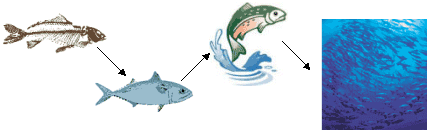
\includegraphics[width=.6\textwidth]{mts-2.png}
\end{center}

Живые организмы, особи, могут объединяться в надсистему. «Надсистема» – это
более или менее организованная совокупность животных или растений, например,
пчелиная семья. Но такого резкого качественного скачка здесь уже не
происходит.


По аналогии с биологическими системами можно трактовать понятие «Техническая
Система» как особый уровень иерархии, при котором система получает возможность
действовать самостоятельно, т.е. уровень живого организма.


Другими словами, «Техническая Система» в технике соответствует уровню живого
организма в природе. В патентной заявке это называется «машина в
работе». Т.е., «система технических объектов» плюс человек-оператор. Например,
карбюратор – это не ТС, а просто – система, совокупность технических
объектов. А вот человек (оператор), стучащий карбюратором по ореху – это ТС с
полезной функцией: очищать орехи от скорлупы. Так и человек с мотыгой – ТС, а
трактор с плугом – нет. Парадокс....

\emph{«Человек» – что это такое в применении к Технической Системе? Что тут трудно
для понимания? }

Наверное, путаница вызывается самой формулировкой вопроса. Психологически
сложно поставить на один уровень человека и колодочный тормоз.

Несомненно, что человек, как часть техносферы, имеет самое прямое отношение к
любой ТС и может быть по отношению к ней в следующих ролевых ситуациях:

\emph{В надсистеме:} 
\begin{itemize}
\item[1.] Пользователем. 
\item[2.] Разработчиком. 
\item[3.] Изготовителем технических объектов системы. 
\item[4.] Лицом, обеспечивающим техническое обслуживание, ремонт и утилизацию
  технических объектов системы.  
\end{itemize}
\emph{В системе:} 
\begin{itemize}
\item[1.] Оператором, главным элементом системы управления. 
\item[2.] Источником энергии. 
\item[3.] Двигателем. 
\item[4.] Трансмиссией. 
\item[5.] Рабочим органом. 
\item[6.] Обрабатываемым объектом. 
\end{itemize}
\emph{В окружающей среде:} 
\begin{itemize}
\item[1.] Элементом окружающей среды. 
\end{itemize}
Пользователь, несомненно, главное лицо. Именно он оплачивает создание ТС,
именно по его воле разработчики и изготовители берутся за дело. Он оплачивает
труд оператора, техническое обслуживание, ремонт и утилизацию технических
объектов системы.

Вторая группа лиц обеспечивает функционирование ТС при работе, испытывает ее
действие на себе.

Третья группа косвенно помогает или препятствует этому процессу, или просто
наблюдает за ним и подвергается воздействию побочных эффектов, возникающих при
работе.


Человек может выполнять несколько ролей одновременно. Например, водитель
собственного автомобиля или человек, пользующийся ингалятором. Или
велосипедист. Он – элемент почти всех систем велосипеда, кроме рабочего органа
(сидения) и трансмиссии (колес и рамы велосипеда).


\emph{Все-таки, получается так, что человек – обязательная часть Технической
Системы.}

Казалось бы, какая разница. Ведь как дойдет до дела, до решения реальных
инженерных задач, то человек быстро уходит за скобки проблемы и работать
приходится на уровне подсистем. Да, но только в тех местах, где согласование и
проход энергии осуществляются между подсистемами, никак не связанными с
оператором. А стоит нам подойти поближе к системе управления, как проблема
взаимодействия человека и технических объектов встает в полный рост.

Взять, к примеру, автомобиль. Свой нынешний облик автомобиль приобрел уже к
концу 70-х годов, когда были изобретены подушки безопасности и надежная
автоматическая коробка передач. Большинство усовершенствований с той поры
направлены только на то, чтобы улучшить управление, безопасность, удобство
обслуживания и ремонта, – т.е., на взаимодействие человека, главной части ТС,
с ее остальными частями.

Грузовик 40-50-х годов имел рулевое колесо диаметром 80 см. Водитель должен
быть очень сильным, чтобы управлять таким автомобилем. А в авиации...
Гигантский самолет 30-х годов «Максим Горький». Чтобы выполнить маневр, за
штурвал должны были тянуть первый и второй пилот вместе. Иногда они звали на
подмогу штурмана и остальной экипаж. Сейчас оператор с помощью усилителей
может управлять гораздо более нагруженными механизмами. Казалось бы, проблема
решена. Ан нет, опять часто забывают про человека... Дело в том, что усилители
не всегда позволяют оператору в полной мере чувствовать поведение управляемого
механизма. Иногда это приводит к авариям.


Например, проблема безопасности движения автомобиля или более «монотонного» в
управлении локомотива. Здесь очень важно, чтобы оператор всегда находился в
бодром, работоспособном состоянии. Проблема эта решается и в надсистеме –
устраняются причины засыпания за рулем, проводится медицинский контроль,
повышается ответственность водителя-оператора. Но все чаще это решается
непосредственно в Технической Системе. Прямо в кабине. Если машинист вовремя
не выключит сигнальную лампочку, остановится двигатель, и поезд
остановится. Или в автомобиле: не поедешь, пока не пристегнешься. Т.е., идет
нормальная обратная связь так же, как и между всеми остальными элементами ТС.


Может быть, одна из причин, по которой это направление совершенствования
технических систем начало активно развиваться только в последние годы, – это
непонимание места человека в их структуре. Вернее, не то, чтобы непонимание,
а.... В общем, разработчик попадает в сложную психологическую
ситуацию. Человек – разработчик нового – по праву ощущает себя творцом. Он не
может до конца прочувствовать того, что такой же человек может быть еще и
оператором, двигателем или рабочим органом – частью механизма, машины,
Технической Системы. Хорошо еще, если это широко используемая ТС, тесно
взаимодействующая с человеком, например, автомобиль. Здесь человек может
являться и разработчиком, и оператором, и пользователем одновременно.

Как и с компьютером. Работать с большинством компьютерных программ сложно даже
сейчас, когда разработчики поняли простую истину, что с программой будет
работать человек-оператор, которому важен результат, а не устройство
программы. Это сейчас появились такие понятия, как «дружественный интерфейс».
А раньше... Зачем далеко ходить, вспомните «Лексикон».

А другие ТС, стоящие, на первый взгляд, далеко от человека.... Имя им легион.
Здесь зачастую и мысль в голову не приходит, что человек – это часть
Технической Системы. А ведь при разработке любой из них необходимо
анализировать взаимодействие составляющих элементов с учетом возможностей
человеческого тела и разума. Иногда это не выполняется.

Мало того, часто не учитываются многие из известных сейчас природных факторов,
влияющих на самочувствие человека, четкость его движений и быстроту реакции. А
вновь открытые психологические факторы, например, «эффект Кассандры» [10]?

И встает страшным грибом Чернобыль, падают авиалайнеры и сталкиваются корабли. 

\emph{А что еще, кроме оператора, нужно для получения готовой к функционированию
Технической Системы?}

Об этом – во второй части этой статьи.

\newpage
\begin{quote}
  Часть II. \url{http://www.gnrtr.ru/Generator.html?pi=200&cp=3}
\end{quote}

\section*{Полный состав минимально работоспособной Технической Системы.}

Есть набор технических объектов, объединенных в систему, есть
человек-оператор. Достаточно ли этого, чтобы Техническая Система выполняла
полезную функцию и удовлетворяла потребность пользователя, или нужно что-то
еще?


Давайте вспомним известный тризовский пример, приведенной в книге Г. Иванова
[11]. Речь идет о российском ученом Капице, посетившем завод Симменса и
Шуккерта по производству генераторов. Хозяева завода показали ему генератор,
не желавший работать, и предложили 1000 марок за исправление. Капица быстро
смекнул, что перекошен и заклинен центральный подшипник, взял молоток и ударил
по корпусу подшипника – генератор заработал.

Смущенные заказчики попросили составить счет за выполненную работу. Капица
написал: \emph{«1 удар молотком – 1 марка, за то, что знал, куда ударить – 999
марок».}


А вот другой пример – из Фенимора Купера [12].

Герои повести убегают от погони, индейцы загнали их в заросли высокой сухой
травы и подожгли ее. Огонь идет стеной, что делать? Старый охотник не
растерялся и поджег траву возле того места, где они стояли. Стена огня пошла
навстречу настигавшему их огненному валу, сжигая топливо для него. Огонь
потух, убегавшие спаслись.

Что есть Техническая Система в одном и другом случае?

В первом примере. Потребность пользователя – запустить генератор. Полезная
функция – выровнять подшипник. Оператор – Капица, система технических объектов
– молоток.

Получается, что Техническая Система – Капица с молотком.

Во втором примере. Потребность пользователя – остановить огонь. Полезная
функция – уничтожить траву (топливо для наступающего огня). Оператор – старый
охотник, система технических объектов – кремень и огниво.

Техническая Система – охотник с кремнем и огнивом.

Что же выходит? Незначительное действие человека-оператора при помощи
примитивных технических средств дали такой грандиозный результат как в первом,
так и втором случае! Неужели это – все? Неужели это полный состав технических
систем, действие которых позволило в первом случае запустить огромный
генератор, а во втором – остановить стену огня?

Нет, это не так.

Самое главное – то, что полностью упускается из виду в предыдущих
рассуждениях, – информационная составляющая.

Действительно, можно безрезультатно стучать молотком по генератору с утра до
ночи. А Капица стучал не как попало, а строго определенным образом. И в этом
случае информационное обеспечение его действий состояло из двух частей:
«умение стучать молотком» и знание, понимание того, «куда надо ударить».

Точно так же и поджечь траву можно было совершенно без толку, и большинство
вариантов могло кончиться плачевно для самого поджигавшего.

Если дальше проанализировать второй пример, то становится очевидным, что само
поджигание сухой травы имеет смысл тогда, когда охотник не только знает, что
ветер может погнать огонь навстречу наступающему огню, но и когда этот самый
ветер, дующий в нужную сторону, есть в наличии.

Следовательно, очень важно знание того «как это сделать?», как выполнить
полезную функцию, используя для этого технические объекты и имеющиеся
вещественно-полевые ресурсы, которые тоже становятся частью ТС на время ее
работы.

Для укомплектования полной минимально работоспособной ТС необходимо учитывать
следующие информационные и материальные составляющие:
\begin{itemize}
\item[1.] Технологический процесс выполнения полезной функции.
\item[2.] Материальные технические и природные объекты и системы разного
  уровня иерархии.
\item[3.] Один или несколько операторов, владеющих совокупностью приемов
  управления материальными объектами и системами.
\item[4.] Вещества и поля, необходимые для работы материальных объектов и
  систем, и продукты их переработки.
\item[5.] Вещества и поля, необходимые для функционирования оператора, и
  продукты их переработки.
\item[6.] Обрабатываемый объект (в отдельных случаях).
\end{itemize}
Полный состав Технической Системы:
\begin{center}
  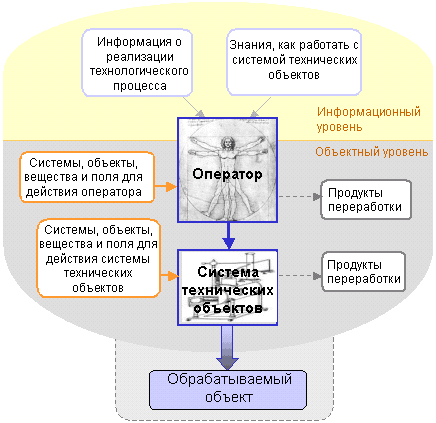
\includegraphics[width=.8\textwidth]{mts-3.png}
\end{center}
Именно в таком составе ТС получает возможность работать везде, в любом месте,
полностью автономно. Даже в невесомости и безвоздушном пространстве.

Данный подход – комплектование ТС всем необходимым для выполнения ее полезной
функции – не отвергает традиционного, но весьма удобен. Собрать все
необходимое для выполнения функции в одну систему и преобразовывать ее,
мысленно отделив от надсистемы. Выполнять любую работу проще, если заранее
приготовить все необходимые материалы, инструменты и чертежи, расположить это
самым удобным образом, чтобы не шарить потом по «мастерской» (Надсистеме),
вспоминая, что же еще надо для обеспечения работоспособности нашей ТС.

То есть, Техническая Система является надсистемой для Системы технических
(материальных) объектов.

Такое понимание ТС перекликается с ее описанием, которое приводит Н.Матвиенко
[8]: \textbf{«Всякая Техническая Система есть совокупность вещественных,
  энергетических и информационных элементов (иначе говоря – вещественных
  частей и деталей, энергетических ресурсов их функционирования и набора
  предписаний, инструкций, команд, сигналов, определяющих последовательность и
  вид взаимодействий вещественных элементов с окружающими системами и между
  собой)».}

Этот подход ставит в центр, в основу Технической Системы, человека-оператора.

При этом «Техническая Система», организуемая человеком, может подразумевать
использование объектных технических или природных элементов – например,
иглоукалывание или перевозка груза, а также вообще обходиться без них – речь
адвоката в суде или танец. От этого иногда мало что меняется. Примером этого
утверждения может служить адвокат, выступающий перед залом с микрофоном или
без него.

А ведь, если разобраться, то человек и есть многофункциональная Техническая
Система. Природа человека двуедина – он обладает способностью мыслить,
моделировать свои действия, принимать решения. И действовать, используя свое
тело для выполнения какой-то работы. Именно здесь и объединяются в одно целое
информационная и материальная составляющие человека.


Человек-оператор включает все основные части ТС и, при условии информационного
и материального обеспечения, может выполнять какие-то функции, согласуясь с
возможностями своего тела. Когда же эти возможности будут исчерпаны, можно
дополнить тело материальными объектами, объединить их в системы и расширить
возможности человека. Начинается нормальный процесс развертывания Технической
Системы. Камень, палка, лопата, экскаватор.... Человек становится все сильнее,
может выполнить все больший объем работы.


А как быть со свертыванием? Ведь человека, кажется, свернуть уже
невозможно. Да, если говорить об свертывании объектов. Но здесь свертывание
идет на информационном уровне.

Например, пора бы полить огород. Можно взять лейку, приспособить шланг,
устроить целую поливальную машину. А можно и просто посмотреть на небо и, если
скоро пойдет дождь, то ничего делать и не надо. То есть, свертывание
происходит на уровне функций, технологических операций. Наконец, на уровне
проектирования сиcтем и процессов. Логическим продолжением этого направления
является и сама ТРИЗ. Ведь понятия «Идеальность», «Идеальный Конечный
Результат» являются одними из базовых понятий этой методики.

Это подметили давным-давно, и редкая сказка обходится без того, чтобы что-то
сделалось само собой, человек добился желаемого безо всяких затрат. Силой
мысли, так сказать, разломать горы. Переместиться во времени и
пространстве. «Техническое задание» на развитие человека в этом направлении
вовсю прописывают фантасты и сказочники. И есть основания думать, что это
направление будет освоено. Левитация, перемещение взглядом предметов, связь на
большие расстояния без всяких технических средств и многое другое – может быть
доступно человеку.


Да, это интересно, но что все вышеписанное дает для преобразования, улучшения
Технической Системы в реальной практике?


\section*{Резкое увеличение количества ресурсов, которые можно применить при
трансформации системы.}

\emph{При традиционном подходе могут использоваться следующие ресурсы:}
\begin{itemize}
\item[1.] Сама система.
\item[2.] Ее подсистемы.
\item[3.] Связи между подсистемами.
\item[4.] Связи между каждой подсистемой и системой.
\end{itemize}
\emph{При предлагаемом подходе количество возможных к использованию ресурсов
  резко увеличивается.  Вот только некоторые из них: }
\begin{itemize}
\item[1.] Сама Техническая Система.
\item[2.] Технологический процесс.
\item[3.] Технологические операции.
\item[4.] Система технических объектов.
\item[5.] Подсистемы системы технических объектов.
\item[6.] Оператор, как мыслящая система.
\item[7.] Тело оператора, как материальная биологическая система.
\item[8.] Органы чувств оператора.
\item[9.] Система навыков оператора.
\item[10.] Отдельные навыки оператора.
\item[11.] Системы, объекты, вещества и поля, потребляемые системой
  технических объектов.
\item[12.] Системы, объекты, вещества и поля, потребляемые оператором.
\item[13.] Связи между Технической Системой и технологическим процессом.
\item[14.] Связи между технологическими операциями и технологическим процессом
\item[15.] Связи между технологическими операциями.
\item[16.] Связи между Технической Системой и технологическими операциями.
\item[17.] Взаимодействие веществ и полей, потребляемых Технической Системой с
  системой технических объектов.
\item[18.] Взаимодействие веществ и полей, потребляемых Технической Системой с
  оператором.
\item[19.] Связи между подсистемами системы технических объектов.
\item[20.] Связи между каждой подсистемой Системы Материальных Объектов и
  системой технических объектов.
\item[21.] Связи между подсистемами системы технических объектов и
  технологическим процессом.
\end{itemize}
........И много других сочетаний элементов Технической Системы.......

Самое время привести несколько примеров. 

\begin{wrapfigure}{l}{.3\textwidth}
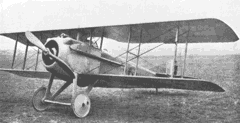
\includegraphics[width=.3\textwidth]{mts-4.png}
\end{wrapfigure}
\paragraph{1. Классический аэроплан.}
Классический аэроплан начала двадцатого века – это два крыла, которые
прикреплялись к фюзеляжу при помощи многочисленных стоек и тросовых
растяжек. Для того, чтобы такой самолет хорошо летал (это было особенно важно
для истребителей), растяжки должны быть правильно натянуты. Поскольку тросы
под нагрузкой вытягивались, растяжки приходилось часто регулировать при помощи
простейшего винтового механизма. К растяжке прикладывалась специальная
линейка, и растяжка оттягивалась с помощью динамометра. О степени натяжения
судили по отклонению растяжки от прямой линии. Процесс этот был весьма
трудоемким и медленным.

Как быть? Как ускорить процесс регулировки растяжек?

По сути дела, нужно было синтезировать новую систему для регулировки
растяжек. Если бы решавшие эту задачу отталкивались только от Системы
Материальных Объектов, применяемых для выполнения этой функции, то решить ее
было бы крайне трудно. Если же вспомнить и учесть, что в системе присутствует
оператор, то количество возможных преобразований значительно
увеличивается. Так, можно решить задачу, использовав органы чувств оператора.

\begin{wrapfigure}{l}{.1\textwidth}
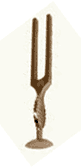
\includegraphics[width=.1\textwidth]{mts-5.png}
\end{wrapfigure}
Действительно, почему не использовать слух, вернее людей с повышенным
тональным слухом? Для регулировки растяжек были приглашены настройщики роялей,
процесс регулировки ускорился во много раз.

Интересно, что поскольку настройщиков роялей было недостаточно, пришлось найти
следующеее решение, в котором прослеживается многократно описанная в ТРИЗ
тенденция: «вытеснение человека из ТС». Регулировку растяжек поручили опять
механикам, но вместо громоздкой линейки и динамометра было предложено
использовать настроенный соответствующим образом камертон.

\paragraph{2. Масляный светильник.}
Трудно представить себе, какую титаническую работу проделали изобретатели,
пытавшиеся заставить хорошо светить масляную лампу. Вся проблема была в плохой
подаче масла к кончику фитиля. Для улучшения подачи создавались многочисленные
пружинные устройства, создающее давление в резервуаре с маслом. Применялись
так же насосы для принудительной подачи масла. То есть, работа шла в рамках
«системы технических объектов» – старались улучшить машину. 
А когда рассмотрели полный состав ТС, стало понятно, что вопрос был не в
устройстве лампы, а в горючем материале. Когда вместо плохо всасывающегося
фитилем масла применили текучий керосин, все проблемы исчезли. 

\paragraph{3. Компьютер.}
Предположим, необходимо пользоваться компьютером в темноте. Если мы будем
трансформировать Систему материальных объектов, то сразу приходит мысль о
светящихся клавишах, лампочках и прочем. Если подумать о Технической Системе,
то ответ очевиден – оператор должен уметь печатать в темноте, помнить
расположение клавишей наизусть.


Что можно сказать в заключение? Сейчас в ТРИЗ и других инновационных методиках
совершенно перепутались понятия «Техническая Система», т.е., система,
\textbf{выполняющая} какую-то функцию, и «Система технических (материальных)
объектов», т.е., система, \textbf{предназначенная} для выполнения какой-то
функции. Как можно меньше вмешиваясь в спор «остроконечников» и
«тупоконечников» (см. эпиграф), я попытался разобраться в этом вопросе.

Не призывая читателя соглашаться со мной, буду рад, если эта попытка анализа
окажется ему в какой-то степени полезной.

Я очень благодарен коллегам В. Леняшину, Г. Северинцу, Е. Новицкой, Н. Хоменко
и беспощадному критику первого варианта статьи В. Сибирякову за помощь в
подготовке данного материала.
\section*{Литература}
\begin{itemize}
\item[1.] B.R. Gaines. «General System research: Quo vadis?» General System
  Yearboor, 24, 1979.
\item[2.] А.А. Богданов. Всеобщая организационная наука. Тектология. Кн. 1. –
  М., 1989. – С. 48.
\item[3.] Г.С. Альтшуллер. Творчество как точная наука.
  \url{http://www.trizminsk.org/r/4117.htm#05}.
\item[4.] А.Ф. Каменев. Технические Системы. Закономерности развития.
  Ленинград, «Машиностроение», 1985.
\item[5.] Г. Альтшуллер, Б. Злотин, А. Зусман. В. Филатов. Поиск новых идей: от
  озарения к технологии. Кишинев, Картя Молдавеняска, 1989. с. 365.
\item[6.] В. Королев. О понятии «система». Энциклопедия ТРИЗ.
  \url{http://triz.port5.com/data/w24.html}.
\item[7.] В. Королев. О понятии «система» (2). Энциклопедия ТРИЗ.
  \url{http://triz.port5.com/data/w108.html}.
\item[8.] Н.Н. Матвиенко. Термины ТРИЗ (проблемный сборник).  Владивосток,
  1991.
\item[9.] Ю.П. Саламатов. Система законов развития техники (Основы теории
  развития Технических систем). INSTITUTE OF INNOVATIVE DESIGN. Красноярск,
  1996.  \url{http://www.trizminsk.org/e/21101000.htm}.
\item[10.] В.А. Свиридов. Человеческий фактор.
  \url{http://www.rusavia.spb.ru/digest/sv/sv.html}.
\item[11.] Г.И. Иванов. Формулы творчества или как научиться изобретать.
  Москва.  «Просвещение». 1994
\item[12.] Ф. Купер. Прерия. 
\end{itemize}

\end{document}
